\documentclass[12pt,a4paper]{article}
\usepackage{ctex}
\usepackage{amsmath,amscd,amsbsy,amssymb,latexsym,url,bm,amsthm}
\usepackage{epsfig,graphicx,subfigure}
\usepackage{enumitem,balance}
\usepackage{wrapfig}
\usepackage{mathrsfs,euscript}
\usepackage[usenames]{xcolor}
\usepackage{hyperref}
\usepackage[vlined,ruled,linesnumbered]{algorithm2e}
\hypersetup{colorlinks=true,linkcolor=black}

\newtheorem{theorem}{Theorem}
\newtheorem{lemma}[theorem]{Lemma}
\newtheorem{proposition}[theorem]{Proposition}
\newtheorem{corollary}[theorem]{Corollary}
\newtheorem{exercise}{Exercise}
\newtheorem*{solution}{Solution}
\newtheorem{definition}{Definition}
\theoremstyle{definition}

\renewcommand{\thefootnote}{\fnsymbol{footnote}}

\newcommand{\postscript}[2]
 {\setlength{\epsfxsize}{#2\hsize}
  \centerline{\epsfbox{#1}}}

\renewcommand{\baselinestretch}{1.0}

\setlength{\oddsidemargin}{-0.365in}
\setlength{\evensidemargin}{-0.365in}
\setlength{\topmargin}{-0.3in}
\setlength{\headheight}{0in}
\setlength{\headsep}{0in}
\setlength{\textheight}{10.1in}
\setlength{\textwidth}{7in}
\makeatletter \renewenvironment{proof}[1][Proof] {\par\pushQED{\qed}\normalfont\topsep6\p@\@plus6\p@\relax\trivlist\item[\hskip\labelsep\bfseries#1\@addpunct{.}]\ignorespaces}{\popQED\endtrivlist\@endpefalse} \makeatother
\makeatletter
\renewenvironment{solution}[1][Solution] {\par\pushQED{\qed}\normalfont\topsep6\p@\@plus6\p@\relax\trivlist\item[\hskip\labelsep\bfseries#1\@addpunct{.}]\ignorespaces}{\popQED\endtrivlist\@endpefalse} \makeatother

\begin{document}
\noindent

%========================================================================
\noindent\framebox[\linewidth]{\shortstack[c]{
\Large{\textbf{Lab07-Graph Exploration}}\vspace{1mm}\\
CS214-Algorithm and Complexity, Xiaofeng Gao, Spring 2018.}}
\begin{center}

\footnotesize{\color{blue}$*$ Name: Hongyi Guo  \quad Student ID: 516030910306 \quad Email: guohongyi@sjtu.edu.cn}
\end{center}

\begin{enumerate}
\item \textbf{BFS Tree:} Similar to DFS, BFS yields a tree, (also possibly forest, but \textbf{just consider a tree} in this question) and we can define \textbf{tree, forward, back, cross} edges for BFS. Denote $Dist(u)$ as the distance between node $u$ and the source node in the BFS tree. Please prove:
    \begin{enumerate}
    \item For both undirected and directed graphs, no forward edges exist in the graph.
    \begin{proof}
    	$\forall$ node $u$ in a graph(could be undirected or directed graphs), any node $v$ which has not been visited by far and has an edge connected to $u$, $v$ should be a child node of $u$ in the BFS tree. While forward edges connect $u$ with its non-child descendants in the BFS tree. So, no forward edges exist in the graph.
    \end{proof}
    
    \item There are no back edges in undirected graph, while in directed graph each back edge $(u,v)$ yields $0\leq Dist(v)\leq Dist(u)$.
    \begin{proof}
    	$\forall$ node $u$ in an undirected graph, when we BFS the graph, every possible edge $(u,v)$ are checked before we visit node $v$. For the edges are undirected, there is no chance to find an edge $(v,u)$ not checked such that $v$ is visited after $u$. Thus, there are no back edges in an undirected graph.
    	
    	In a directed graph, assume $(u,v)$ is a back edge. Then $v$ is an ancestor of $u$. We know BFS finds the shortest path between the source node and any tree node in the graph with all edges' length equal to $1$. So $v$ must in the shortest path between $u$ and the source node in the BFS tree. So, $Dist(u)=Dist(v)+\min\{path(v,u)\}\geq Dist(v)\geq 0$.
    \end{proof}

    \item For undirected graph, each cross edge $(u,v)$ yields $Dist(v)=Dist(u)$ or $|Dist(v)-Dist(u)|=1$, while for directed graph, each cross edge $(u,v)$ yields $Dist(v)\leq Dist(u)+1$.
    \begin{proof}
    	As we already know, BFS always finds the shortest path in the graph with all edges' length equal to $1$. 
    	
    	In a directed graph, for each cross edge $(u,v)$, if $Dist(v)>Dist(u)+1$, there exists a path $(src\rightarrow u\rightarrow v)$ whose length is $Dist(u)+1$, which contradicts that the shortest length of path between $v$ and source node is $Dist(v)$. So, $Dist(v)\leq Dist(u)+1$.
    	
    	In an undirected graph, for the same reason, we have $Dist(v)\leq Dist(u)+1$. Since $(v,u)$ is also a cross edge, we also have $Dist(v)\leq Dist(u)+1$. Together, $Dist(v)=Dist(u)$ or $Dist(v)=Dist(u)\pm1$.
    \end{proof}
    \end{enumerate}

\item \textbf{Second-best Minimum Spanning Tree:} Let $G=(V,E)$ be an undirected, connected graph whose weight function is $w: E\rightarrow \mathbb{R}^{+}$. Assume that $|V|\leq |E|$ and the weight of each edge is distinct. Let $\mathcal{T}$ be the set of all spanning trees of $G$, and let $T^{\prime}$ be the minimum spanning tree of $G$. The \textbf{second-best minimum spanning tree} is a spanning tree $T^{\prime\prime}$ such that $w(T^{\prime\prime})=\min_{T\in \mathcal{T}\slash\{T^\prime\}} w(T)$, where $w(T)=\sum_{e\in T} w(e)$.

\begin{enumerate}
\item Prove that $G$ contains $u,v,x,y \in V$, $(u,v)\in T^{\prime}$ and $(x,y)\notin T^{\prime}$, such that $(T^{\prime}\slash(u,v))\cup(x,y)$ is a second-best minimum spanning tree.
\begin{proof}
	We know $T^{\prime}$ must have at least one edge different from $T$. We consider every edge $(u,v)$ in $T$. Suppose we delete $(u,v)$. Then the original graph is divided into two connected components $C_1$ and $C_2$. We need to find an edge $(u_1,v_1)$ which connects $C_1$ and $C_2$. If there is no edge satisfying this condition except $(u,v)$, we choose another edge in $T$ and try again. Otherwise, we replace $(u,v)$ with $(u_1,v_1)$ and get a new spanning tree $T_1$. $w(T_1)\leq w(T)$.
	
	Then, we try to replace another edge $(u_2,v_2)$ of $T_1$ and get $T_2$. Assume $w(T_2)>w(T_1)$. Suppose after we remove $(u_2,v_2)$, $G$ is divided into two connected components $C_3$ and $C_4$. The new edge $(u_3,v_3)$ must connect this two components and its weight is larger than $(u_2,v_2)$. Then we replace $(u_2,v_2)$ with $(u_3,v_3)$ in $T$ and get $T_3$. We have $w(T_3)=w(C_3)+w(u_3,v_3)+w(C_4)>w(C_3)+w(u_2,v_2)+w(C_4)$ which contradicts that $T$ is minimum spanning tree. So, after we replace another edge in $T_1$, the total weight must go down. So, to get the second-best minimum spanning tree, we only need to replace one edge of $T$ and try it on every edge to find the largest new spanning tree $T^\prime$.
\end{proof}

\item \label{Problem:2b}Let $T$ be a spanning tree of $G$, for any two vertices $u,v\in V$, let $\max [u,v]$ denote the edge with maximum weight on the simple path between $u$ and $v$ in $T$. Please design an algorithm with time complexity $O(|V|^2)$ which computes $\max [u,v]$ for all $u,v\in V$ and $u \neq v$, given $T$. Briefly explain your idea and write your algorithm in \emph{pseudo code}.
\begin{solution}
	For every vertex $u$, we DFS $T$ with $u$ as the source. And compute $max[u,v]$ during this procedure.
	
	\begin{minipage}[t]{0.9\textwidth}
	\begin{algorithm}[H]
		\BlankLine
		\SetKwFunction{dfs}{DFS}
		\SetKwBlock{DFS}{}{}
		\SetKwInOut{Input}{input}
		\SetKwInOut{Output}{output}
		\caption{}
		\Input{$T$: $\forall u$, give the weight of all its edges $w[u,v]$ in $T$}
		\Output{$max[u,v]$, $\forall u,\forall v$}
		\BlankLine
		\dfs($src,u$)
		\DFS{
			\ForEach{$v$ connected to $u$}{
				\If{$visited[v]=false$}{
					$visited[v]\leftarrow true$\;
					$max[src,v]\leftarrow\max(max[src,u],w[u,v])$\;
					\dfs($src,v,maxv$)\;
				}
			}
		}
		\BlankLine
		\ForEach{$u$ in $T$}{
			$max[u,u]\leftarrow 0$\;
			$visited[1\dots n]\leftarrow false$\;
			$visited[u]\leftarrow true$\;
			\dfs($u$, $u$)\;
		}
	\end{algorithm}
	\end{minipage}
\end{solution}

\item Explain your idea to compute the second-best minimum spanning tree of $G$ based on your analysis of Problem \ref{Problem:2b}, and analyze the time complexity of your idea.
\begin{solution}
	First, we compute the MST of $G$, denoted by $T$, and next for all $u$ and $v$ in $G$, compute $max[u,v]$ in $T$.
	
	Then, for every edge $(u^\prime,v^\prime)$ in $G$ but not in $T$, we replace the edge weighted $max[u^\prime,v^\prime]$ with $(u^\prime,v^\prime)$. The weight of $T$ will increase by $\delta(u^\prime,v^\prime)=w(u^\prime,v^\prime)-max[u^\prime,v^\prime]$. So for all $(u',v')$'s, we have to compute $\delta(u^\prime,v^\prime)$ and find the minimal $\delta_{min}$. The weight of second minimum spanning tree of $G$ is $w(T)+\delta_{min}$.
	
	The time complexity of computing MST is $O(|E|\log|E|)$ supposing we use Kruskal algorithm and that of computing $max[u,v]$ is $O(|V|^2)$ from Problem 2b. The last step is $O(|E|)$. So the total time complexity is $O(|E|\log|E|+|V|^2)$.
\end{solution}
\end{enumerate}

\item \textbf{Counting Connected Components:} The file \emph{Data-CCC.txt} represents a graph $G=(V,E)$. Inside, the first row shows $|V|$ (left) and $|E|$ (right). There are $|E|$ rows after the first row. Each row represents an edge, where the left element is the ID of starting vertex while the right is that of ending vertex. The ID of vertices is from $0$ to $|V|-1$. Please solve problems below.
    \begin{enumerate}
    \item Suppose $G$ is an undirected graph, Please write code by C/C++ which outputs \emph{the number of connected components (CC)} and \emph{the largest CC}. Source code should be named as {\color{red}\emph{Code-CC.cpp}}, and you need to write a file named {\color{red}\emph{Output-CC-Your ID.txt}} (Exp. Output-CC-5140219173.txt), in which the first row is the number of CC, and the second row is the ID of vertices in the largest CC sorted in \textbf{increasing} order.
    \item Suppose $G$ is a directed graph, Please write code by C/C++ which outputs \emph{the number of strongly connected components (SCC)} and \emph{the largest SCC}. Source code should be named as {\color{red}\emph{Code-SCC.cpp}}, and you need to write a file named {\color{red}\emph{Output-SCC-Your ID.txt}} (Exp. Output-SCC-5140219173.txt), in which the first row is the number of SCC, and the second row is the ID of vertices in the largest SCC sorted in \textbf{increasing} order.
    \item {\color{red}(Optional Subquestion with Bonus)} Visualize the above two graphs. Please use a \emph{metanode} to denote a CC/SCC, and the \emph{radius} of a metanode should be positively proportional to the size of the corresponding CC/SCC.
    
    \begin{center}
    	CC
    	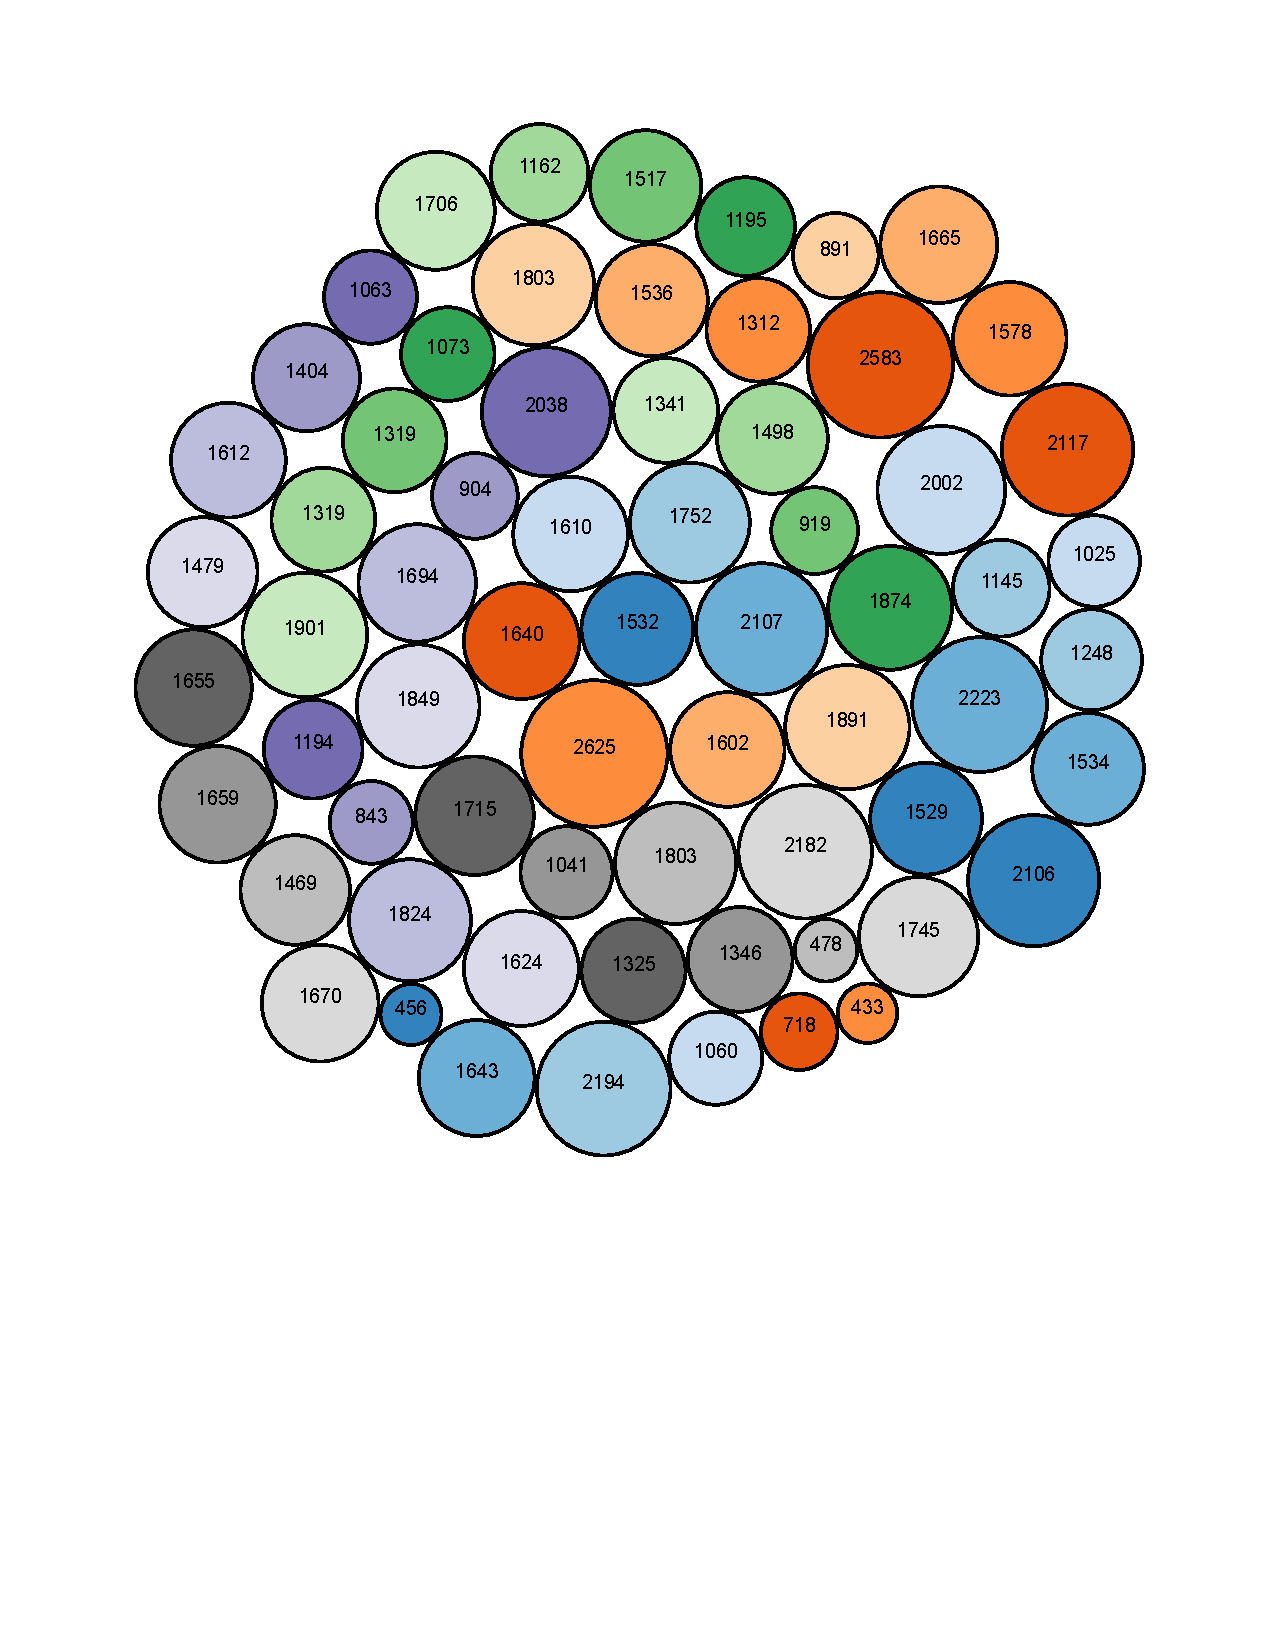
\includegraphics[width=0.6\textwidth]{CC.pdf}
    \end{center}
	\begin{center}
		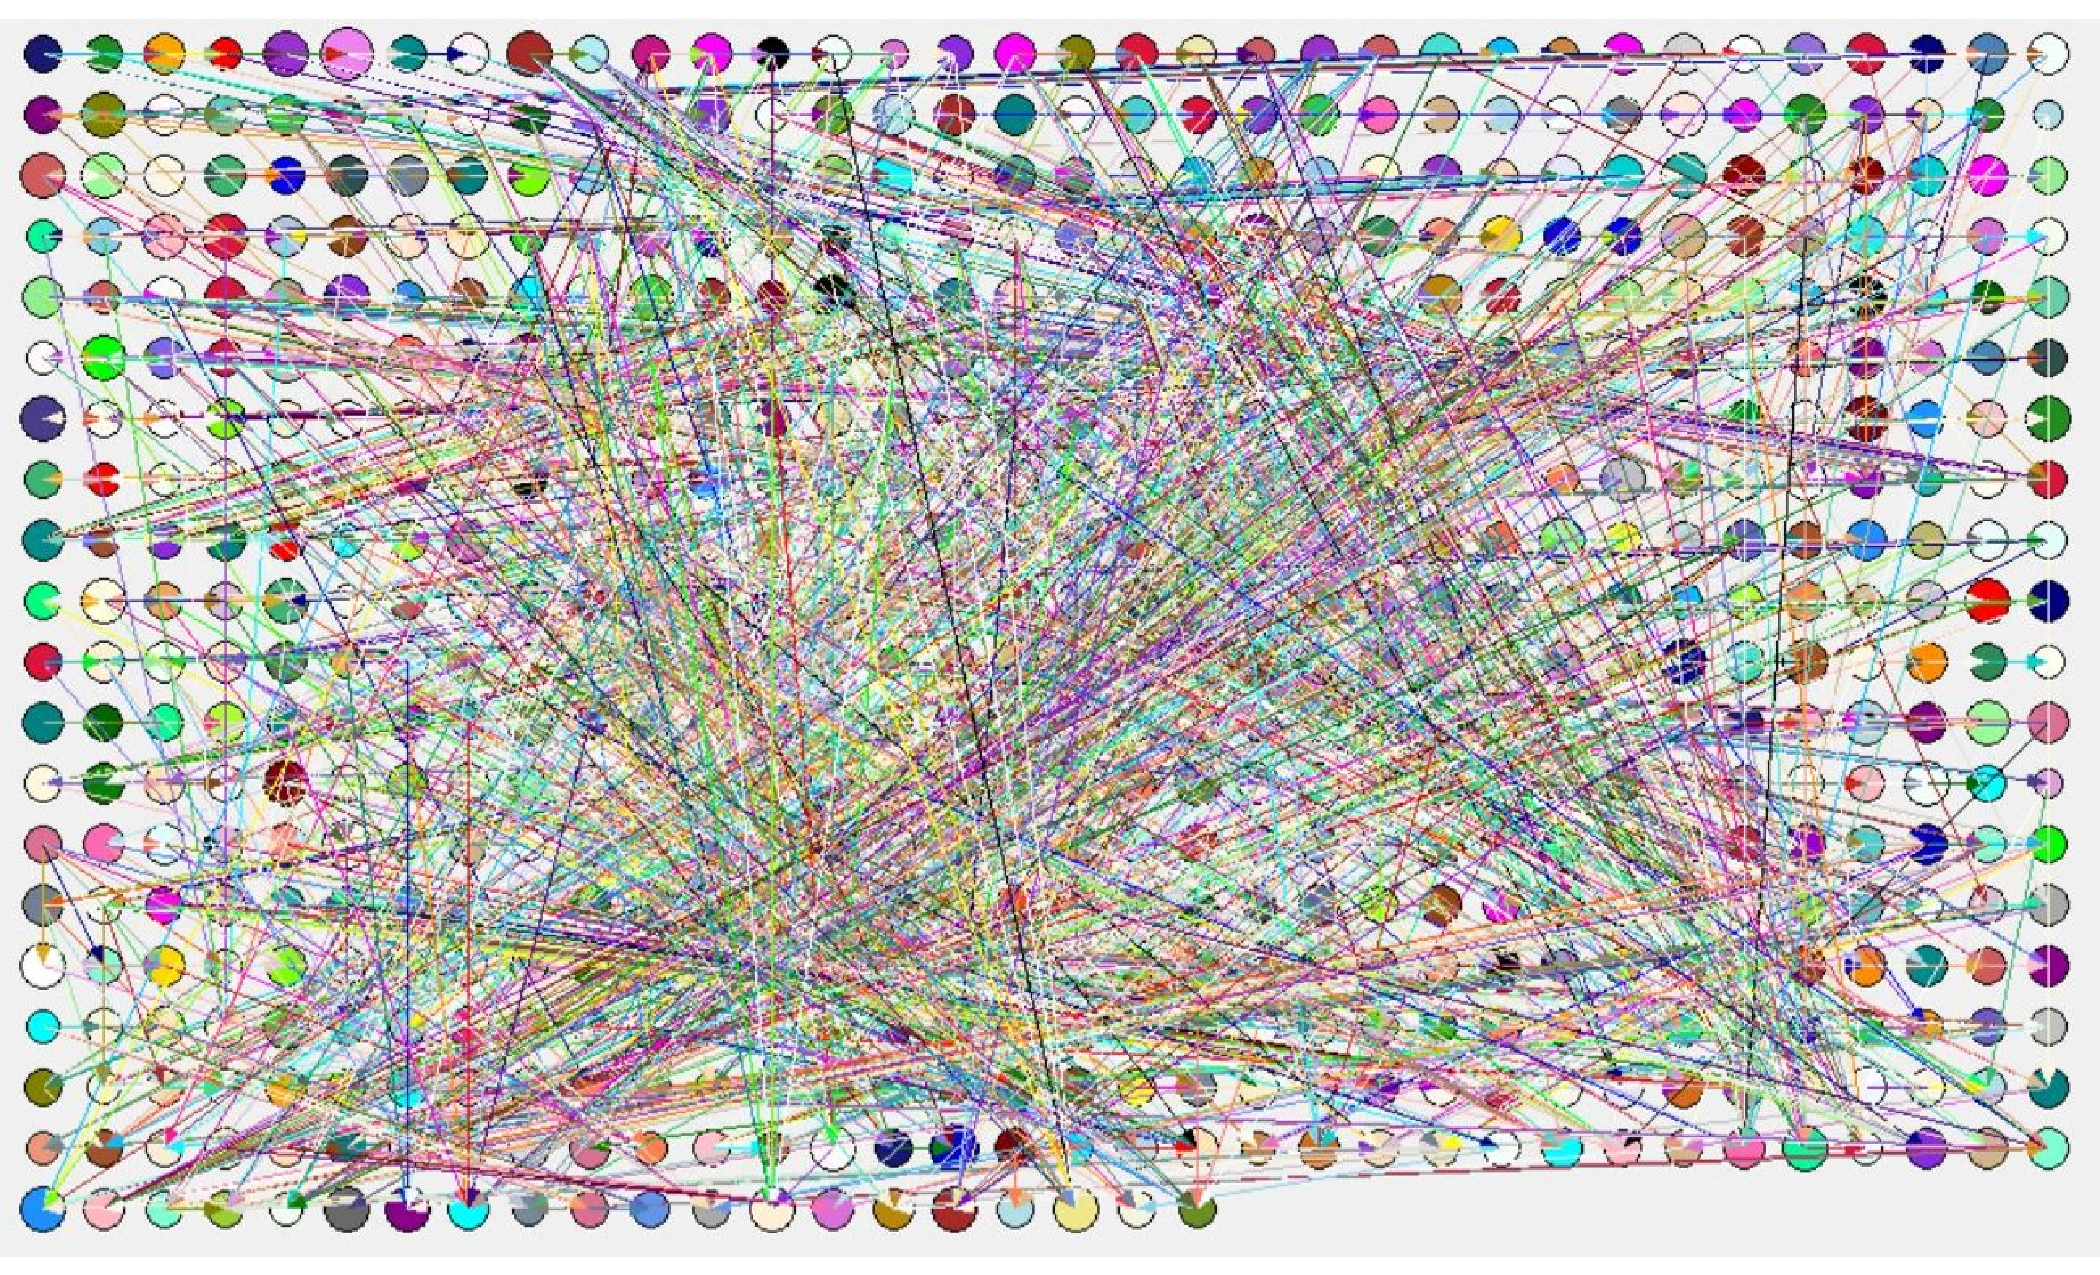
\includegraphics[width=0.9\textwidth]{SCC.pdf}
		SCC
	\end{center}

    \end{enumerate}
\end{enumerate}

\textbf{Remark:} Please include {\color{red}.pdf}, {\color{red}.tex}, {\color{red}.cpp} and {\color{red}.txt} files in your .rar files with standard names.

\qquad \quad \quad Please do \textbf{NOT} include \emph{Data-CCC.txt} in your uploaded file.

%========================================================================
\end{document}
